\documentclass[12pt]{article}
\usepackage{graphicx}
\usepackage{hyperref}
\usepackage{float}
\usepackage[margin=1in]{geometry}
\usepackage{subcaption}

\title{CarND Advanced Lane Finding Project Writeup}
\author{Tiffany Huang}
\date{\today}

\begin{document}
\maketitle


\section{Advanced Lane Finding Project}
This project consists on the following steps/tasks:
\begin{itemize}
\item {Compute the camera calibration matrix and distortion coefficients given a set of chessboard images.}
\item {Apply a distortion correction to raw images.}
\item {Use color transforms, gradients, etc., to create a thresholded binary image.}
\item {Apply a perspective transform to rectify binary image ("birds-eye view").}
\item {Detect lane pixels and fit to find the lane boundary.}
\item {Determine the curvature of the lane and vehicle position with respect to center.}
\item {Warp the detected lane boundaries back onto the original image.}
\item {Output visual display of the lane boundaries and numerical estimation of lane curvature and vehicle position.}
\end{itemize}
My project code can be found here: \url{https://github.com/tahuang/Advanced_Lane_Finding}. Next, I will consider each of the rubric points individually and describe how I addressed each point in my implementation.

\section{Camera Calibration}
I calculated the correct camera matrix and distortion coefficients using several calibration chessboard images and the OpenCV \texttt{calibrateCamera} function. The code can be found in section 1 of \texttt{lane\_finding.ipynb}. The following is an example of a successfully undistorted calibration image:

\begin{figure}[h]
\centering
\begin{subfigure}{.5\textwidth}
  \centering
  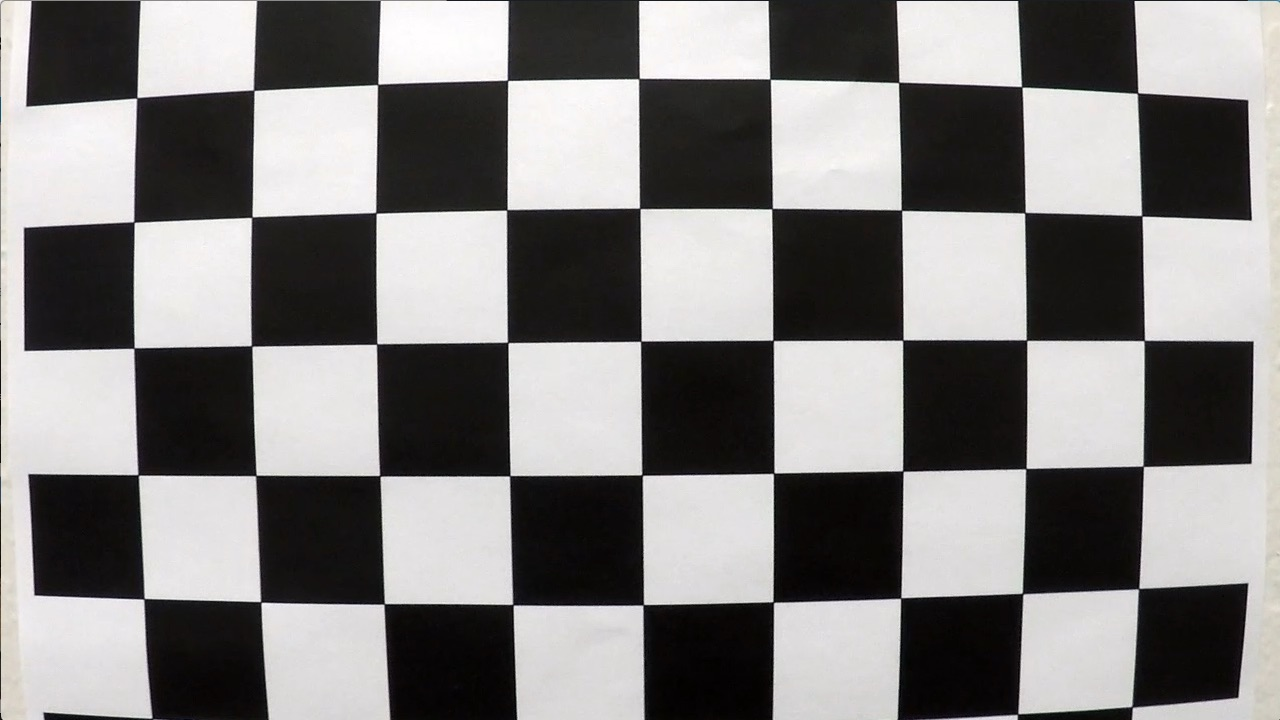
\includegraphics[width=1\linewidth]{../camera_cal/calibration1.jpg}
  \caption{Original calibration image}
\end{subfigure}%
\begin{subfigure}{.5\textwidth}
  \centering
  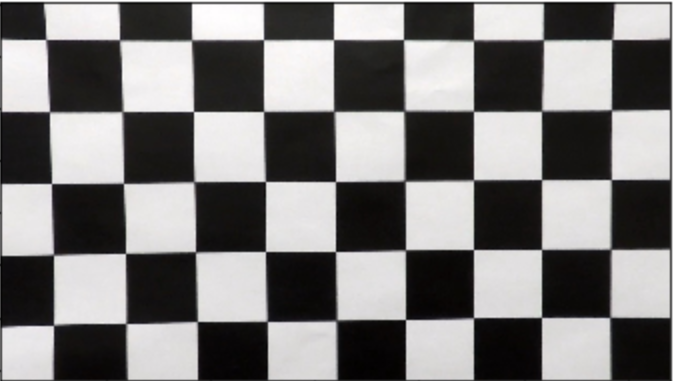
\includegraphics[width=1\linewidth]{undistorted_calibration.png}
  \caption{Undistorted calibration image}
\end{subfigure}
\caption{Example of distortion corrected calibration image}
\label{fig:distortion_correction_calibration}
\end{figure}

\section{Pipeline}

The code to run the entire pipeline is in the last section of \texttt{lane\_finding.ipynb} titled "Pipeline".

\subsection{Distortion Correction}
Distortion correction was done using the camera calibration parameters found in the previous step and the OpenCV \texttt{undistort} function. The code can be found in section 2 of \texttt{lane\_finding.ipynb} and line 21 of the last cell. An example of a distortion corrected image is below. The undistorted image doesn't look much different because there was not too much distortion in the original image.

\begin{figure}[h]
\centering
\begin{subfigure}{.5\textwidth}
  \centering
  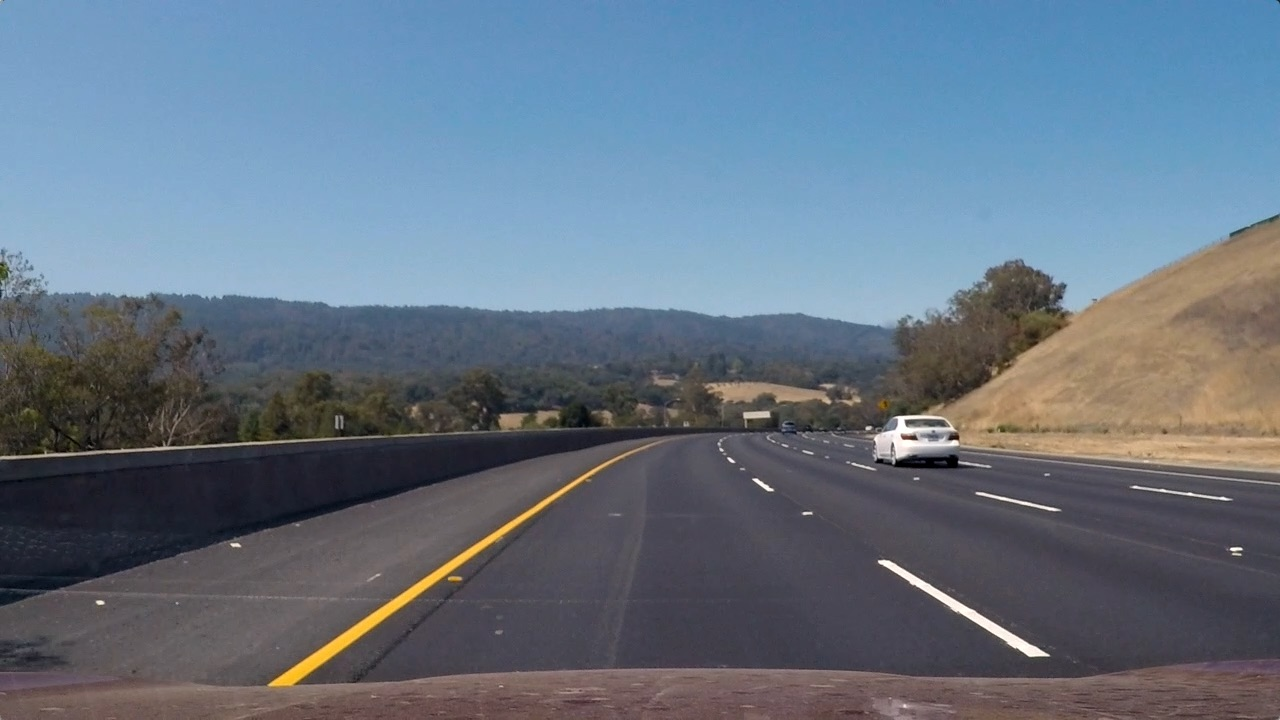
\includegraphics[width=1\linewidth]{../test_images/test3.jpg}
  \caption{Original image}
\end{subfigure}%
\begin{subfigure}{.5\textwidth}
  \centering
  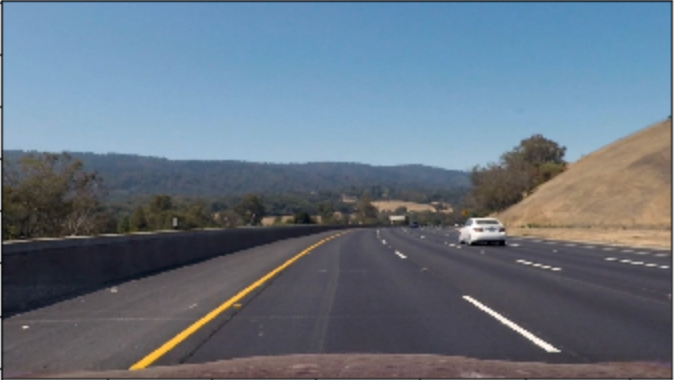
\includegraphics[width=1\linewidth]{undistorted_test.png}
  \caption{Undistorted image}
\end{subfigure}
\caption{Example of distortion corrected image}
\label{fig:undistorted_img}
\end{figure}

\subsection{Thresholded Binary Image}
Next, I created a thresholded binary image by first Gaussian blurring the image to reduce noise. I then applied the $Sobel_x$ and $Sobel_y$ operators and a HLS color threshold to the image. Table~\ref{tab:threshold_table} shows the thresholds I used for each filter. I then combined all of the binary images from each method to create a combined threshold. Figure~\ref{fig:threshold_img} shows an example of the combined output. The code for the thresholding is on lines 26-33 of the last cell and in the cells under section 3 of \texttt{lane\_finding.ipynb}. After thresholding, I also cropped a region of interest to focus on the important pixels and reduce noise and outliers (code on line 38 of last cell).

\begin{table}[ht]
\begin{tabular}{|c | c | c | c |}
\hline
\textbf{Operator} & \textbf{Kernel Size} & \textbf{Min Threshold} & \textbf{Max Threshold} \\ \hline
Absolute Value of Sobel in X direction & 15 & 40 & 90 \\ \hline
Absolute Vallue of Sobel in Y direction & 15 & 40 & 150 \\ \hline
Magnitude of Sobel & 15 & 20 & 150 \\ \hline
Direction of Sobel & 15 & 0.4 & 1.2 \\ \hline
HLS Saturation & N/A & 190 & 255 \\ \hline
\end{tabular}
\caption{Filter Thresholds}
\label{tab:threshold_table}
\end{table}

\begin{figure}[h]
\centering
\begin{subfigure}{.5\textwidth}
  \centering
  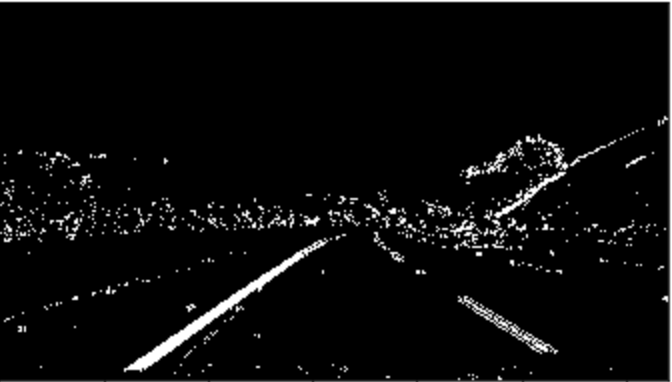
\includegraphics[width=1\linewidth]{thresholded_test.png}
  \caption{Combined thresholded image}
\end{subfigure}%
\begin{subfigure}{.5\textwidth}
  \centering
  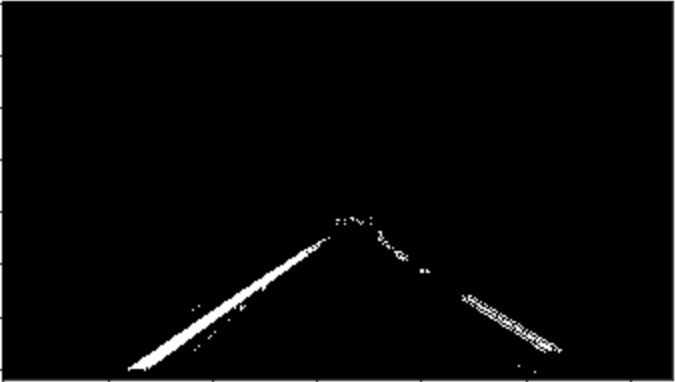
\includegraphics[width=1\linewidth]{roi_test.png}
  \caption{Region of interest image}
\end{subfigure}
\caption{Example of thresholded binary image}
\label{fig:threshold_img}
\end{figure}

\subsection{Perspective Transform}
The next step was to apply a perspective transform on the image to transform the lane markings to a bird's eye view. This transform will help us to calculate the lane curvature. I used OpenCV's \texttt{warpPerspective} function and the code can be found in section 4, lines 4-7 of the second cell under the "Pipeline" section, and line 43 of the last cell. The following is an example of the perspective transformation:

\begin{figure}[h]
\centering
\begin{subfigure}{.5\textwidth}
  \centering
  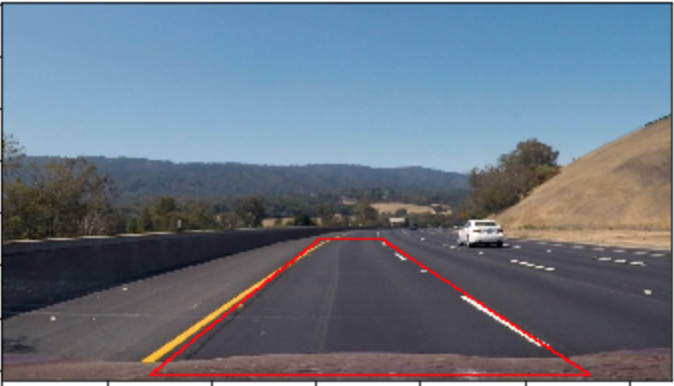
\includegraphics[width=1\linewidth]{src_pts.png}
  \caption{Before perspective transform}
\end{subfigure}%
\begin{subfigure}{.5\textwidth}
  \centering
  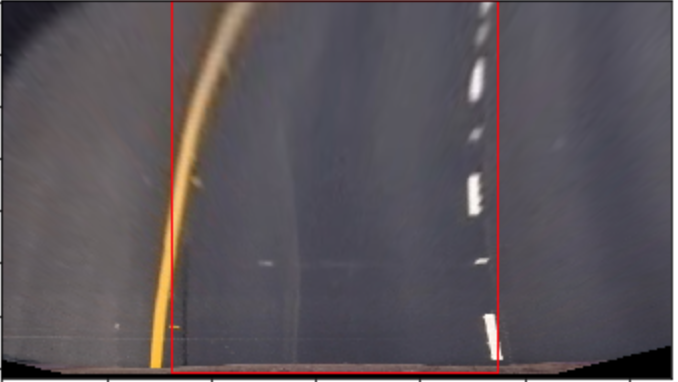
\includegraphics[width=1\linewidth]{warped_src_pts.png}
  \caption{After perspective transform}
  \label{fig:perspective}
\end{subfigure}
\caption{Example of perspective transform}
\end{figure}

\subsection{Fitting a Polynomial to Lane Pixels}
Once I have transformed the image to a bird's eye view, I detect the lane pixels in the image and fit a quadratic function to the pixels. For the first image, I used the convolution approach, where I sliced the image into 9 vertical layers and first found the maximum convolution signal with the a small window template to find the starting places for the left and right lane. Then, for each following layer, I search in a margin around the past left lane centroid and the past right centroid, find the maximum convolution signal, and mark that as the left lane centroid and right lane centroid. If no lane pixels are found in the layer, I just keep the past left and right centroids. Then, I search for nonzero pixels around the lane centroids and fit a quadratic function to the pixels using \texttt{np.polyfit}. The code for this is in section 5 of \texttt{lane\_finding.ipynb} and lines 50-51 of the last cell.

For every following image, I simply do a margin search for nonzero pixels around the best polynomial fit so far for the left and right lanes. Then, I fit a quadratic function to the new pixels with \texttt{np.polyfit}. The code for this is in section 5 of \texttt{lane\_finding.ipynb} and lines 52-53 of the last cell. Figure~\ref{fig:lane_pixels} shows an example of the lane centroid search result for the first image and an example of fitting a quadratic to the lane pixels.

\begin{figure}[h]
\centering
\begin{subfigure}{.5\textwidth}
  \centering
  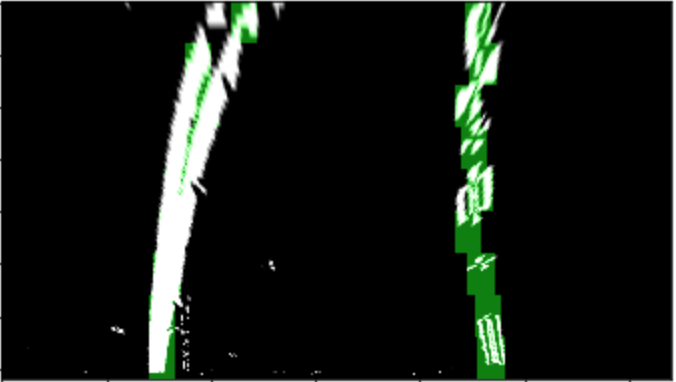
\includegraphics[width=1\linewidth]{window_test.png}
  \caption{Convolution window search result}
\end{subfigure}%
\begin{subfigure}{.5\textwidth}
  \centering
  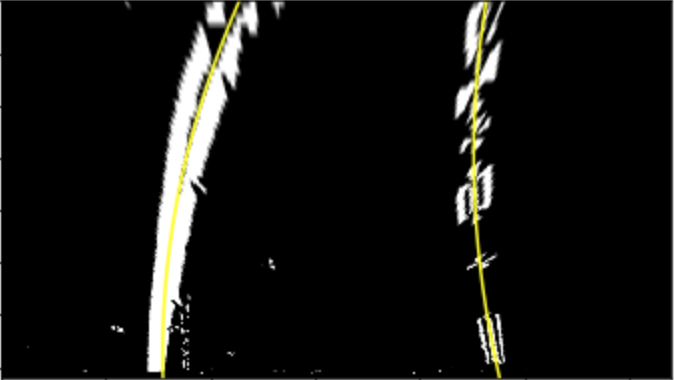
\includegraphics[width=1\linewidth]{polyfit_test.png}
  \caption{Polynomial fitting result}
\end{subfigure}
\caption{Example of lane pixel detection and polynomial fitting}
\label{fig:lane_pixels}
\end{figure}

\subsection{Radius of Curvature and Offset from Center}
Next, I calculate the radius of curvature by transforming the lane pixels into meters, refitting a polynomial to the lanes in meters, and calculating the radius as follows:
\begin{equation}
r = \frac{[1+(\frac{dx}{dy})^2]^\frac{3}{2}}{|\frac{d^2x}{dy^2}|}
\label{eq:radius}
\end{equation}

With a quadratic fit for the lanes, where $x = ay^2 + by + c$, Eq.~\ref{eq:radius} then becomes:
\begin{equation}
r = \frac{[1+(2ay + b)^2]^\frac{3}{2}}{|2a|}
\end{equation}

The code for radius curvature calculation is in section 6 of \texttt{lane\_finding.ipynb} and line 56 of the last cell.

The offset of the car from the center of the lane was calculated by finding the halfway point between the first left lane pixel and the first right lane pixel, comparing this to the width of the image divided by 2, and then converting to meters. It is assumed that the camera is mounted at the center of the car. The code for finding the offset can be found in section 6 and line 57 of the last cell of \texttt{lane\_finding.ipynb}. For example, for the image displayed in Fig~\ref{fig:perspective}, the radius of curvature was 508.06 m for the left lane boundary and 599.81 m for the right lane boundary and the offset from center was -0.222 m.

\subsection{Plotting the Lane Area}
Finally, the last step was to warp the lane boundaries back onto the image. I do this by creating a polygon of the left and right points using OpenCV's \texttt{fillPoly} function. Then, I draw the polygon on a warped blank image and warp the polygon image back to the original image perspective with OpenCV's \texttt{warpPerspective} function and the inverse perspective matrix found earlier in the pipeline. I then combine this image with the original image using the OpenCV \texttt{addWeighted} function. An example with the lane fit plotted on the original image is shown below:

\begin{figure}[h]
\centering
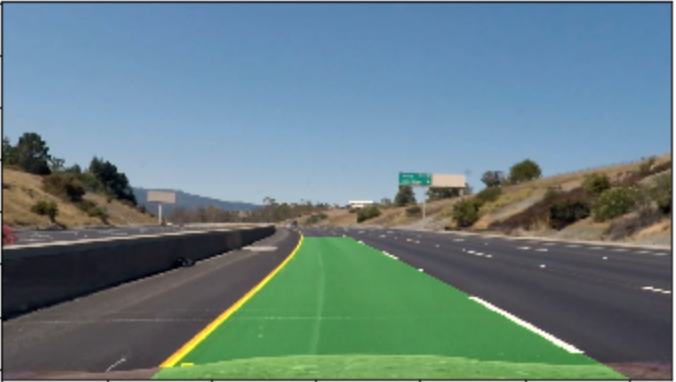
\includegraphics[scale=1]{lane_test.png}
\caption{Warping lane boundaries back onto image}
\label{fig:lane_plot}
\end{figure}

\section{Output Video}
My output video can be found in \texttt{lane\_video.mp4}.

\section{Discussion}
My pipeline would fail in drastically different lighting conditions than the one given for this project since I use filters on image gradients and color saturation thresholding. Any sort of lighting that would make it difficult to distinguish the lane markings from the road such as driving at nighttime or having part of the road heavily shaded would cause a failure. A possible solution to this would be to incorporate another sensor like Lidar that could pick up the lane marking reflectors on the road.

Another possible failure case is if the lane markings are very windy or strangely shaped. In these cases, my quadratic fit of the lane pixels would fail since the lane does not follow a quadratic model. I could use a higher degree of polynomial for the polynomial fit to accommodate potential shapes, but this may not be a good solution because higher degree polynomials may introduce more noise and fluctuation in the fit. Additionally, if the lanes don't have well-defined and nicely painted lane markings, my filters would not work very well and it would be difficult to extract the lane boundaries. Once again, another sensor that could detect lane reflectors or some other kind of reasoning such as following a vehicle in front of you would help with this issue.

Finally, another confusing case would be if the car changed lanes. This would cause some confusion in the lane boundary tracking and the car would need to take some time to reset and recover the new lane boundaries. A possible solution would be to have the car send a signal to the pipeline when it performs a lane change so that the pipeline can immediately reset. 
 
\end{document}
